\chapter{Over Sensor Maritime}
Sensor Maritime is een bedrijf dat zicht focust op research en development in de maritieme sector. Sensor Maritime is één van de vier bedrijven die deel uitmaken van de Sensor Groep, deze groep bestaat uit Sensor Maritime, Sensor BV, Sensor Partners, en Vision Partners. Wat deze bedrijven met elkaar gemeen hebben, is dat deze allemaal gefocust zijn op het ontwikkelen van nieuwe technologieën met verschillende sensoren. Sensor Maritime heeft één kantoor in Vught. Het bedrijf bestaat uit vier mensen en heeft drie afdelingen:
\begin{enumerate}
	\item Sales
	\item Service
	\item Research en Development
\end{enumerate}
Tijdens de afstudeerstage is de stagiair alleen betrokken bij Research and Development.
\newline

\noindent Sensor Maritime is gespecialiseerd in het ontwikkelen van sensoren. De specifieke focus op het ontwikkelen van sensorsystemen voor binnenvaartschepen. De klanten van Sensor Maritime zijn dan ook kapiteins van binnenvaartschepen, een voorbeeld van een klant van Sensor Maritime is te zien op afbeelding \ref{fig:customer_sensor_maritime}.
\begin{figure}[h!]

	\centering

	\label{fig:customer_sensor_maritime}
	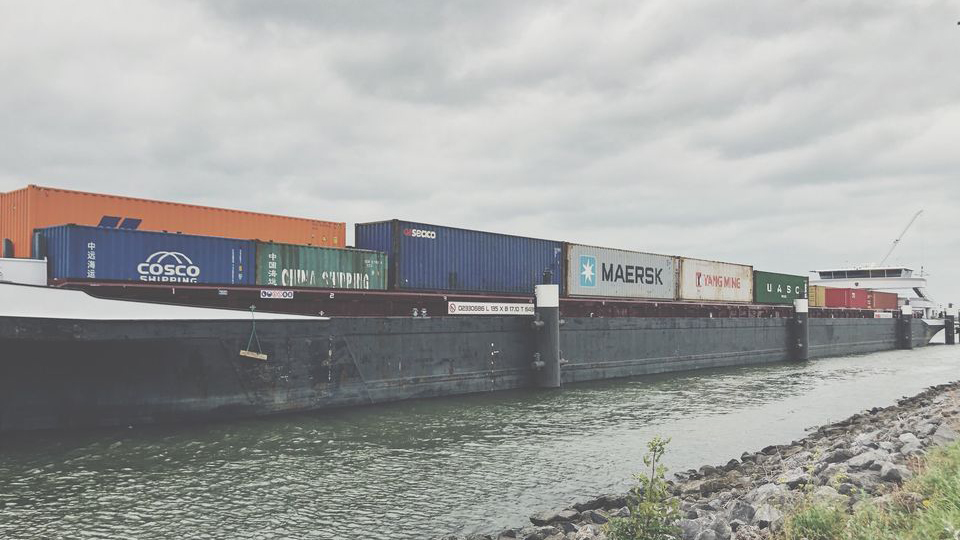
\includegraphics[width=0.7\linewidth]{about/binnevaart.jpg}
	\caption{Voorbeeld van type klant Sensor Maritime}

\end{figure}

\noindent Een project waar Sensor Maritime momenteel bezig mee is, is bijvoorbeeld een systeem om objecten aan de zijkanten van een schip te kunnen detecteren en deze te tekenen op een scherm. Daarnaast is ook met een systeem om objecten aan de voorkant van een schip te kunnen detecteren, en een systeem om te kunnen detecteren of een schip met de stuurhut onder een brug door kan.
